%%%%%%%%%%%%%%%%%%%%%%%%%%%%%%%%%%%%%%%%%%%%%%%%%%%%%%%%%%%%%%%%%%%%%%%
%% template for II2202 report
%% original 2015.11.24
%% revised  2016.08.23
%%%%%%%%%%%%%%%%%%%%%%%%%%%%%%%%%%%%%%%%%%%%%%%%%%%%%%%%%%%%%%%%%%%%%%%
%

\title{Designing Deixis Usage in Real-time Collaborative Drawing}
\author{
        \textsc{Jiayao Yu}
            \qquad
        \textsc{Yumin Hong}
        \mbox{}\\
        \normalsize
            \texttt{jiayaoy}
        \textbar{}
            \texttt{yumin}
        \normalsize
            \texttt{@kth.se}
}
\date{\today}

\documentclass[12pt,twoside]{article}

\usepackage[paper=a4paper,dvips,top=1.5cm,left=1.5cm,right=1.5cm,
    foot=1cm,bottom=1.5cm]{geometry}
\usepackage{booktabs}

%\usepackage[T1]{fontenc}
%%\usepackage{pslatex}
\renewcommand{\rmdefault}{ptm} 
\usepackage{mathptmx}
\usepackage[scaled=.90]{helvet}
\usepackage{courier}
%
\usepackage{bookmark}

\usepackage{fancyhdr}
\pagestyle{fancy}

%%----------------------------------------------------------------------------
%%   pcap2tex stuff
%%----------------------------------------------------------------------------
 \usepackage[dvipsnames*,svgnames]{xcolor} %% For extended colors
 \usepackage{tikz}
 \usetikzlibrary{arrows,decorations.pathmorphing,backgrounds,fit,positioning,calc,shapes}

%% \usepackage{pgfmath}	% --math engine
%%----------------------------------------------------------------------------
%% \usepackage[latin1]{inputenc}
\usepackage[utf8]{inputenc} % inputenc allows the user to input accented characters directly from the keyboard
\usepackage[swedish,english]{babel}
%% \usepackage{rotating}		 %% For text rotating
\usepackage{array}			 %% For table wrapping
\usepackage{graphicx}	                 %% Support for images
\usepackage{float}			 %% Suppor for more flexible floating box positioning
\usepackage{color}                       %% Support for colour 
\usepackage{mdwlist}
%% \usepackage{setspace}                 %% For fine-grained control over line spacing
%% \usepackage{listings}		 %% For source code listing
%% \usepackage{bytefield}                %% For packet drawings
\usepackage{tabularx}		         %% For simple table stretching
%%\usepackage{multirow}	                 %% Support for multirow colums in tables
\usepackage{dcolumn}	                 %% Support for decimal point alignment in tables
\usepackage{url}	                 %% Support for breaking URLs
\usepackage[perpage,para,symbol]{footmisc} %% use symbols to ``number'' footnotes and reset which symbol is used first on each page

%% \usepackage{pygmentize}           %% required to use minted -- see python-pygments - Pygments is a Syntax Highlighting Package written in Python
%% \usepackage{minted}		     %% For source code highlighting

%% \usepackage{hyperref}		
\usepackage[all]{hypcap}	 %% Prevents an issue related to hyperref and caption linking
%% setup hyperref to use the darkblue color on links
%% \hypersetup{colorlinks,breaklinks,
%%             linkcolor=darkblue,urlcolor=darkblue,
%%             anchorcolor=darkblue,citecolor=darkblue}

%% Some definitions of used colors
\definecolor{darkblue}{rgb}{0.0,0.0,0.3} %% define a color called darkblue
\definecolor{darkred}{rgb}{0.4,0.0,0.0}
\definecolor{red}{rgb}{0.7,0.0,0.0}
\definecolor{lightgrey}{rgb}{0.8,0.8,0.8} 
\definecolor{grey}{rgb}{0.6,0.6,0.6}
\definecolor{darkgrey}{rgb}{0.4,0.4,0.4}
%% Reduce hyphenation as much as possible
\hyphenpenalty=15000 
\tolerance=1000

%% useful redefinitions to use with tables
\newcommand{\rr}{\raggedright} %% raggedright command redefinition
\newcommand{\rl}{\raggedleft} %% raggedleft command redefinition
\newcommand{\tn}{\tabularnewline} %% tabularnewline command redefinition

%% definition of new command for bytefield package
\newcommand{\colorbitbox}[3]{%
	\rlap{\bitbox{#2}{\color{#1}\rule{\width}{\height}}}%
	\bitbox{#2}{#3}}

%% command to ease switching to red color text
\newcommand{\red}{\color{red}}
%%redefinition of paragraph command to insert a breakline after it
\makeatletter
\renewcommand\paragraph{\@startsection{paragraph}{4}{\z@}%
  {-3.25ex\@plus -1ex \@minus -.2ex}%
  {1.5ex \@plus .2ex}%
  {\normalfont\normalsize\bfseries}}
\makeatother

%%redefinition of subparagraph command to insert a breakline after it
\makeatletter
\renewcommand\subparagraph{\@startsection{subparagraph}{5}{\z@}%
  {-3.25ex\@plus -1ex \@minus -.2ex}%
  {1.5ex \@plus .2ex}%
  {\normalfont\normalsize\bfseries}}
\makeatother

\setcounter{tocdepth}{3}	%% 3 depth levels in TOC
\setcounter{secnumdepth}{5}
%%%%%%%%%%%%%%%%%%%%%%%%%%%%%%%%%%%%%%%%%%%%%%%%%%%%%%%%%%%%%%%%%%%%
%% End of preamble
%%%%%%%%%%%%%%%%%%%%%%%%%%%%%%%%%%%%%%%%%%%%%%%%%%%%%%%%%%%%%%%%%%%%

\renewcommand{\headrulewidth}{0pt}
\lhead{II2202, Fall 2017, Period 1-2}
%% or \lhead{II2202, Fall 2016, Period 1}
\chead{Final project report}
\rhead{\date{\today}}

\makeatletter
\let\ps@plain\ps@fancy 
\makeatother

\setlength{\headheight}{15pt}
\begin{document}

\maketitle


\begin{abstract}
\label{sec:abstract}

Humans are used to using deixis in face-to-face collaborations during the evolution over thousands of years, to facilitate communication by shortening and simplifying dialogue. However, in geographically separated Computer-Supported Collaborative Work (CSCW), it is awkward to use deixis due to lack of contextual information. In this paper, we placed our focus on real-time collaborative drawing, analyzed deixis usage in face-to-face collaboration and CSCW respectively based on our field experiment and statistical modeling. In the end we proposed some interaction patterns to optimize deixis usage in real-time collaborative drawing, with scalability to general CSCW groupware designs. 
\\
\\
\textbf{Keywords}: deixis; collaborative drawing; CSCW; interaction design.

\end{abstract}

%%\clearpage

\selectlanguage{english}
\tableofcontents

% \section*{List of Acronyms and Abbreviations}
% \label{list-of-acronyms-and-abbreviations}

% This document requires readers to be familiar with terms and concepts described in \mbox{RFC~1235} \cite{john_ioannidis_coherent_1991}. For clarity we summarize some of these terms and give a short description of them before presenting them in next sections.

% \begin{basedescript}{\desclabelstyle{\pushlabel}\desclabelwidth{10em}}
% \item[IPv4]					Internet Protocol version 4 (RFC~791 \cite{postel_internet_1981})
% \item[IPv6]					Internet Protocol version 6 (RFC~2460 \cite{deering_internet_1998})
% \end{basedescript}


\clearpage
\section{Introduction}
\label{sect:introduction}
%% Longer problem statement
%% General introduction to the area

% It was conjectured in \cite{john_ioannidis_coherent_1991} that multicasting
% could provide gains by \ldots.

% See also \cite{a_new_synchronization_protocol_for_sqlite_databases},
% the paper \cite{anand_kannan_n-ary_2012}, 
% and the book \cite{brent_s._baxter_standard_1982}.

In natural face-to-face collaborations, collaborators mutually perceive information not only from explicit resulting expressions on shared media, such as writing and drawing on paper, but also from implicit accompanying indications through the collaboration process, such as facial expressions and hand gestures. To be more specific, those implicit accompanying indications are categorizes as deictic words, demonstration action, and manifesting actions \cite{gutwin2002descriptive}. When collaborators refer to an object on their shared media, they often use deixis to indicate their reference. It is widely used in face-to-face collaborations, while its semantic meaning is strongly dependent on situated context, which are often missing in Computer-Supported Collaborative Work (CSCW). Proper deixis usage in CSCW can help collaborators gain contextual information and facilitate their mutual communications. However, there were insufficient interaction designs for CSCW shared media groupwares to empower collaborators to use deixis as freely as face-to-face collaborations. Though there were different research frameworks on deixis usage, we still can sense the gap between theoretical research and industrial practices, especially for real-time collaborative drawing groupware designs.

(placeholder: One more paragraph here summarizing our achieved contributions.)

\subsection{Literature study}
\label{sect:literature}

xxxxx xxxx xxxx 

\subsection{Research questions, hypotheses}
\label{sect:questions}

Our overall research aims to find out where and why are the differences of deixis usage happening in face-to-face collaboration and CSCW two setups, then to know via interaction design how to address the deficiency in CSCW caused by differences with the counterparts in face-to-face collaboration. We assumed collaborators have different needs to use deixis in two setups in terms of expression purpose and significance, and they have different ways to use deixis in two setups even for the same expression purpose. Based on that, we scoped our research questions as 1) how are the differences on the needs of deixis usage in face-to-face collaboration and CSCW, in terms of expression purpose and significance, 2) how do collaborators express deixis distinctly in two setups, and 3) how are the current groupware designs that support deixis usage in CSCW and what could be improved. 


\section{Methods}
\label{sec:method}

\subsection{Collaborative drawing field experiment}
\label{sect:collaborative}
To investigate where and why the differences happen in face-to-face collaboration and CSCW this two setups, we started off a user study in field experiment manner to yield ecologically valid results. In sum, we setup realistic test stage to simulate collaborative drawing environment in creative work settings, sampled a pair of test subjects from targeted user group, signed consent forms with them to allow us to video-record and publish our research results, instructed test subjects tasks one by one, assisted them to perform tasks only if they requested so, interviewed them right after the field experiment, then instantly analysed data using affinity diagram, later encoded field experiment data from videos, and statistical modelled in the end.

\subsubsection{User tasks design}

Since we aimed to research on the differences caused by collaborative drawing task platforms, we set this - face-to-face collaboration or CSCW - as the only controlled variable throughout our field experiment. 

We designed two sets of three-task for face-to-face collaboration and CSCW settings respectively, two sets have equivalent task designs but with different description and requirement. The three tasks in each set are puzzles, room layout design and storyboard design based on room layout design. We wanted to encourage collaboration and researched in creative work setting, so we chose the tasks that support collaborative interactions as much as possible and afford big design spaces for creativity. Detailed description on tasks is in appendix\ref{appdx:user tasks}. 

\subsubsection{Test subject sampling}

To understand the rationale behind collaboration behaviours, we chose in-depth video-recording analysis after the field experiment, but because of its characteristic time-consumption, we only invited a pair of test subjects. Through the one-hour field experiment, we still got considerable amount of video materials for our analysis.

This two test subjects both are male with proficiency in ICT devices usage, they did not know each other before, thus they had to use clear deixis expression without any prior tacit agreement. To research cross experienced designer and novice designer, only one of our test subjects has design experience, whilst the other doesn't have. 

\subsubsection{Test stage setup}

The field experiment were conducted in two groupwork rooms in KTH Kista to minimize environmental interference. We experimented face-to-face collaboration session first, then had our test subjects take a 15-minute break and come back to CSCW session, so that they could familiarize with our test first with their natural face-to-face collaboration setting while utilising their full set of deixis expression, then went to CSCW setting with rested fresh minds.

In face-to-face collaboration session, test subjects puzzled and drew using papers and pens on the same desk shoulder-by-shoulder; in CSCW session, they were in two different rooms connected by a video call, and individually drew on iPad touch screens using RealTime Board app.

\subsection{Groupware interaction design}
\label{sect:groupware}
After user study analysis, we started thinking what could be improved for the deficiency in CSCW caused by the deixis usage differences with face-to-face communication.

\section{Results and Analysis}
\label{sec:results}

\subsection{Field experiment}
By video observation, we recorded every episode about using deixis. Each episode contains unstructured data such as action and utterance, so at first, we encode those raw data into finite categories in terms of action mode (action categorization), deixis reference (what did test subjects mean), and deixis role (why did test subject use deixis). Our detailed encoding framework and framework is shown in Table \ref{framework}.

\begin{table}
\begin{tabular}{p{6cm}p{6cm}p{4.6cm}}
\hline
Action Mode & Deixis Reference & Deixis Role\\
\hline
Observe & Object & Express ideas\\
Describe & Scale & Coordinate with actions\\
Select & Position & Seek confirmation\\
Point generally & Event & Reflection \\
Point specifically & Time & Take example \\
Move & & \\
Draw & & \\
Input data & & \\
\hline
\end{tabular}
\caption{Field experiments video recording encoding framework}
\label{framework}
\end{table}

%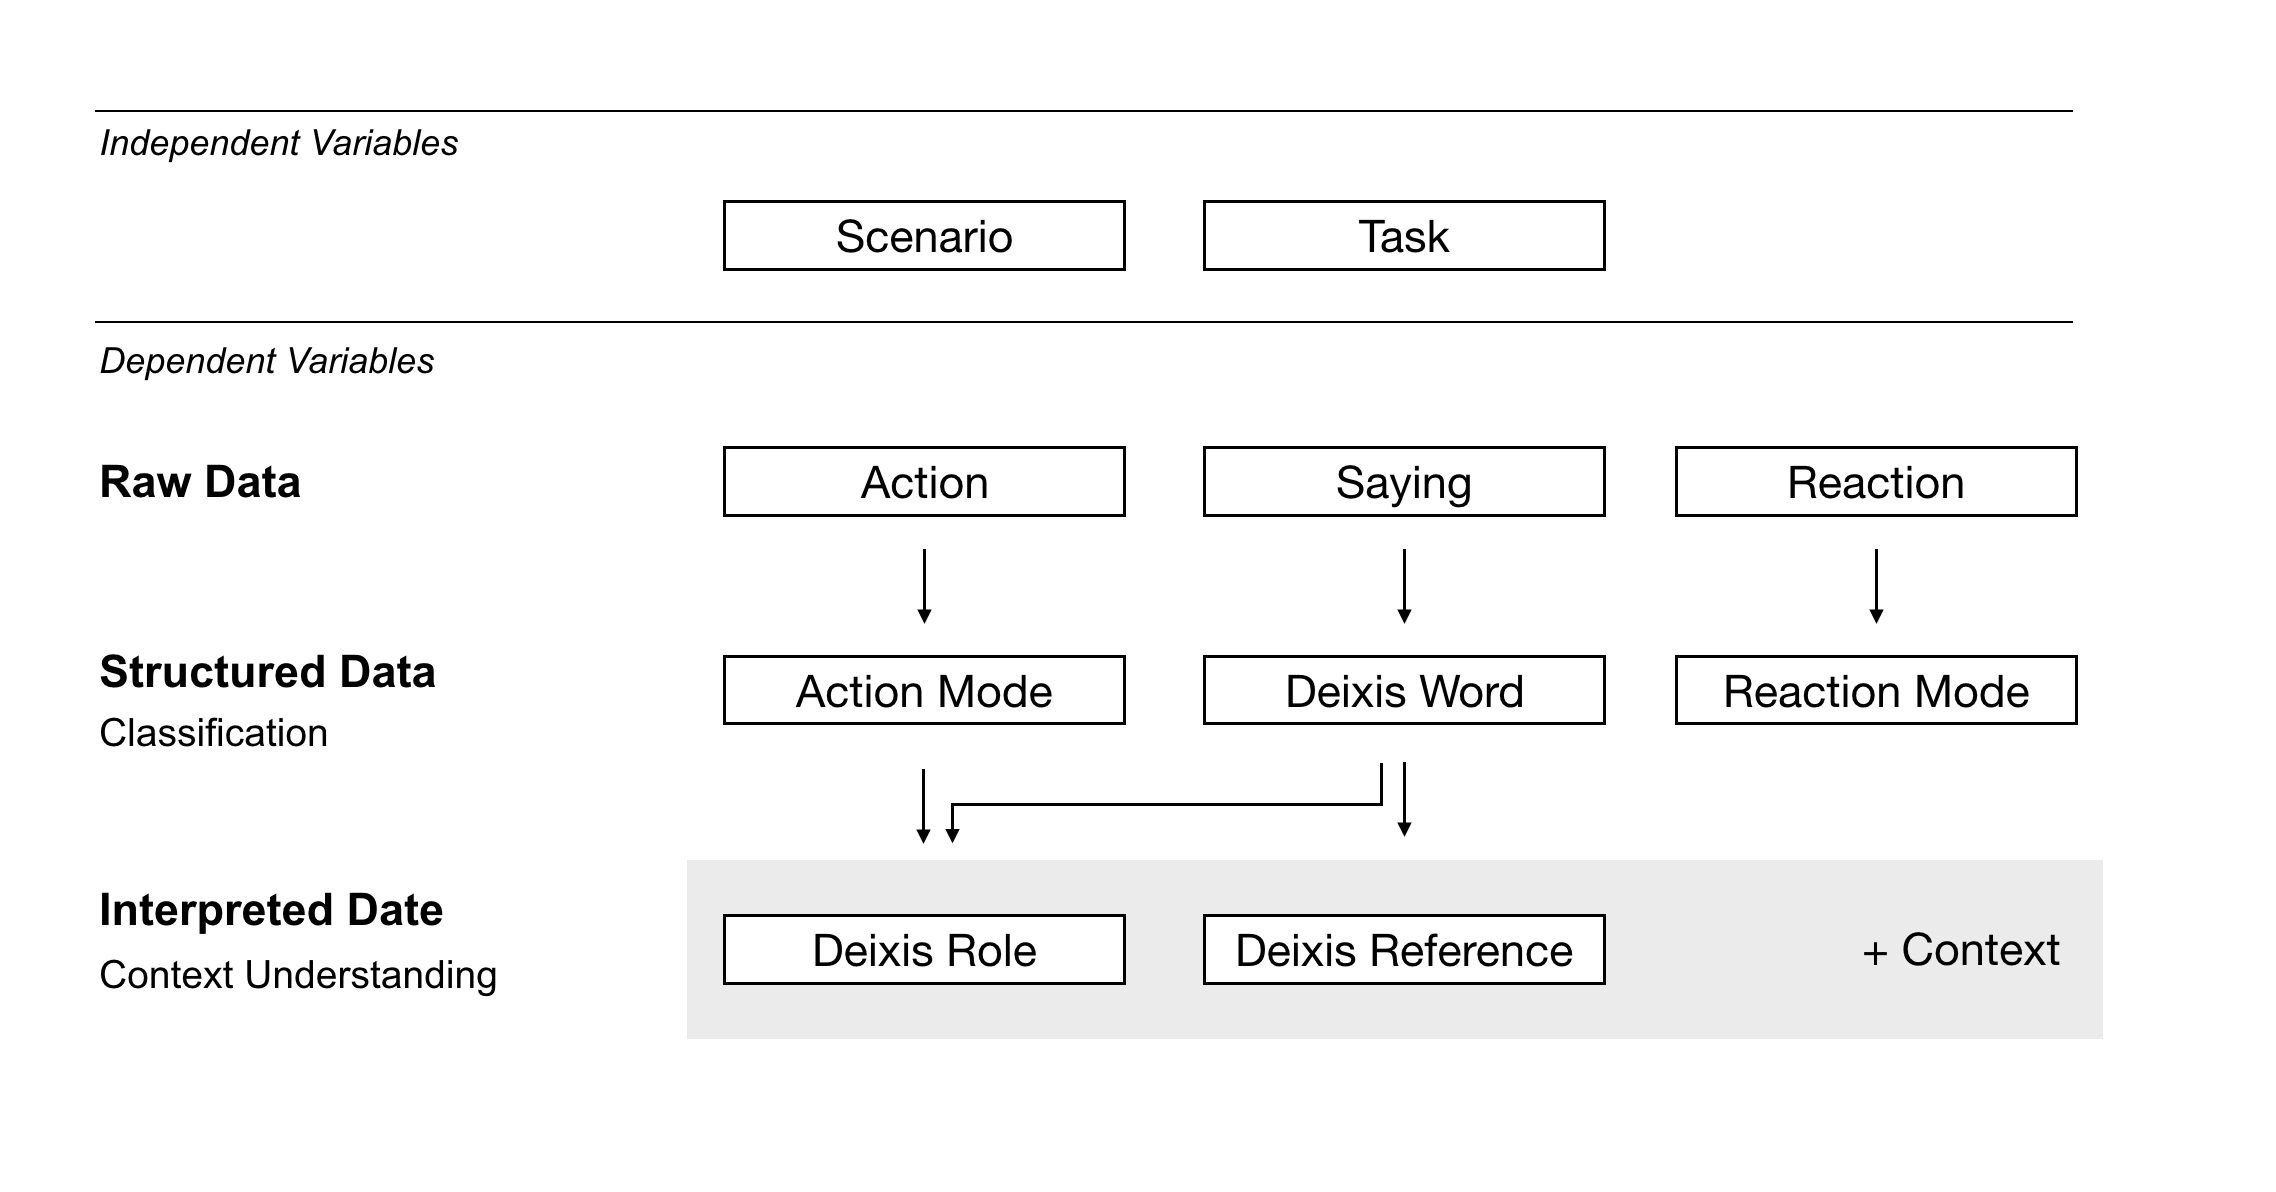
\includegraphics[width = 1\textwidth]{data_processing.png}
We conclude our result as following questions: What is the difference of Action mode in different tasks, between face-to-face scenario and CSCW scenario? What is the difference of deixis reference in different tasks, between face-to-face scenario and CSCW scenario? And what is the difference of deixis role in different tasks, between face-to-face scenario and CSCW scenario?

\begin{figure}
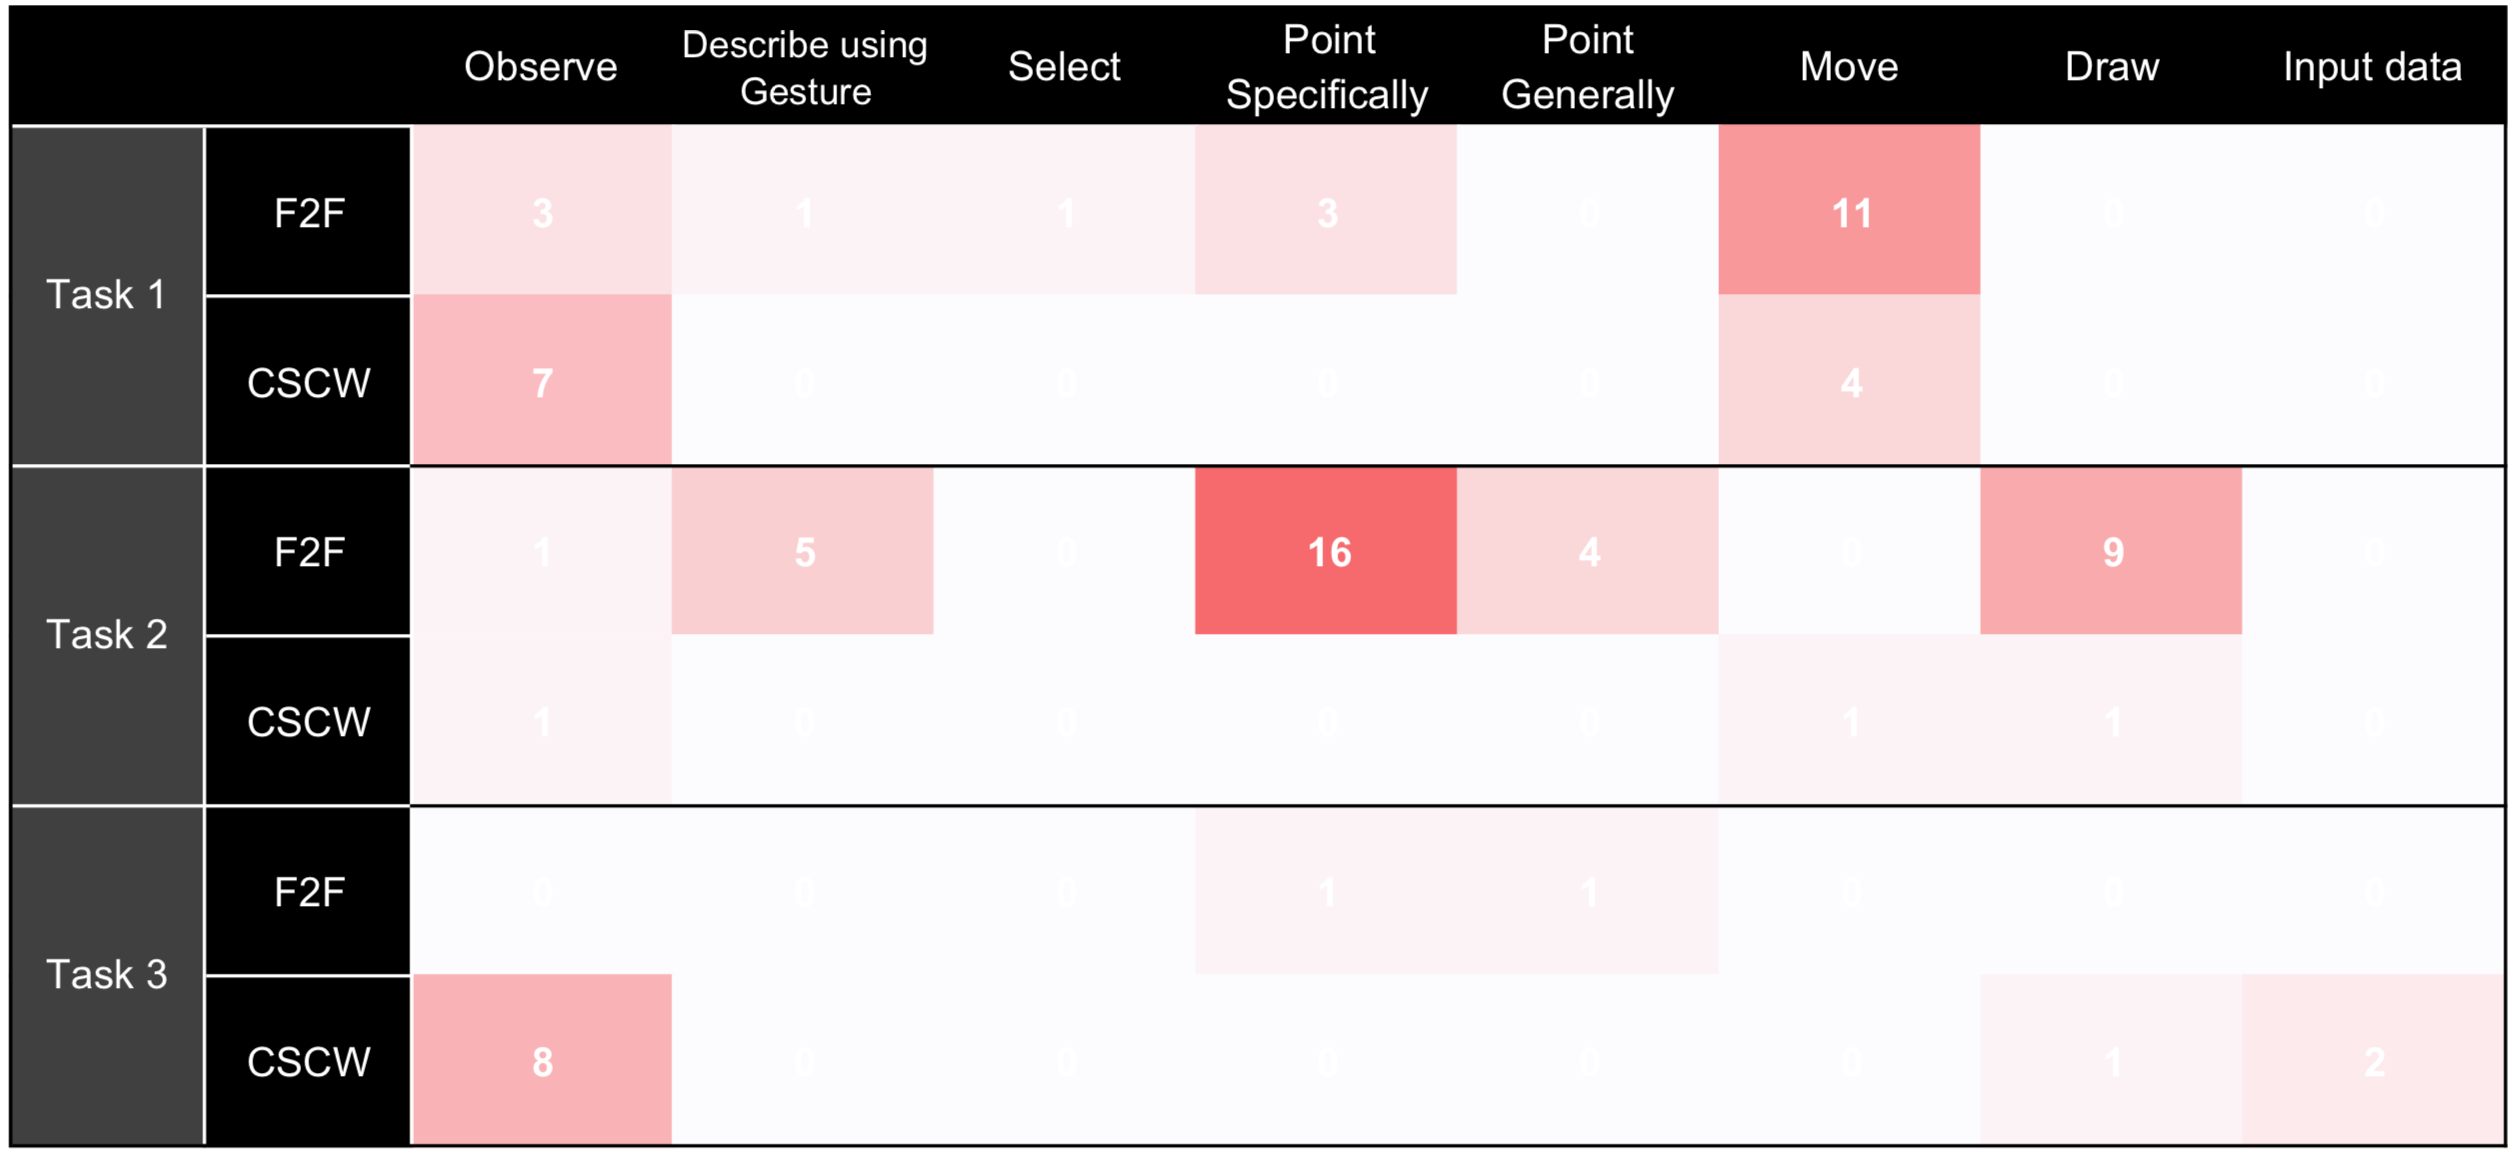
\includegraphics[width = 0.522\textwidth]{action_mode_a.png}
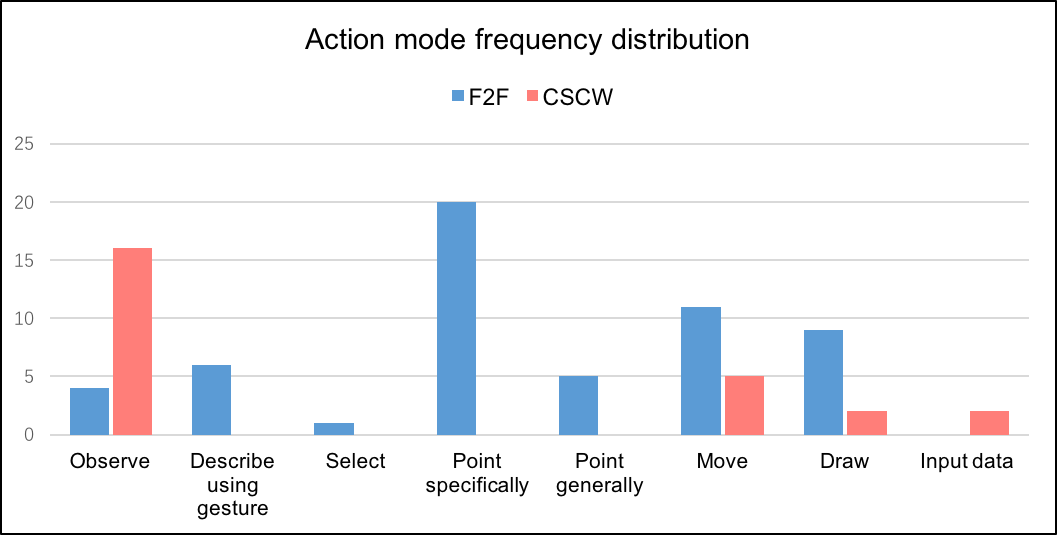
\includegraphics[width = 0.476\textwidth]{action_mode_b.png}
\caption{Action mode frequency distribution}
\label{actionmode}
\end{figure}

Figure \ref{actionmode} shows distribution of action mode when using deixis. These figures illustrate obviously that frequency of using deixis in CSCW is far lower than in face-to-face in the entire video record. In task 1 and task 2, collaborators use more deixis in face-to-face communication, but in task 3, deixis used in CSCW is a little more than in face-to-face.  Collaborators using deixis with observing in CSCW is more frequent than in face-to-face, which is only difference comparison among all action modes. As shown in figure x(b), pointing (includes point specifically and point generally) is the most frequent action compared with deixis. Moving is highly frequent too, but it happens only in task 1. Pointing, selecting and describing with gesture are never used to assist deixis expression in CSCW. In addition, we find that in task 1 and task 2, collaborators tend to operate elements directly when use deixis. For example, one says “these two...” meanwhile move those two element to other place; one says “the door size should be this” while he draw a line to illustrate his meaning.

\begin{figure}
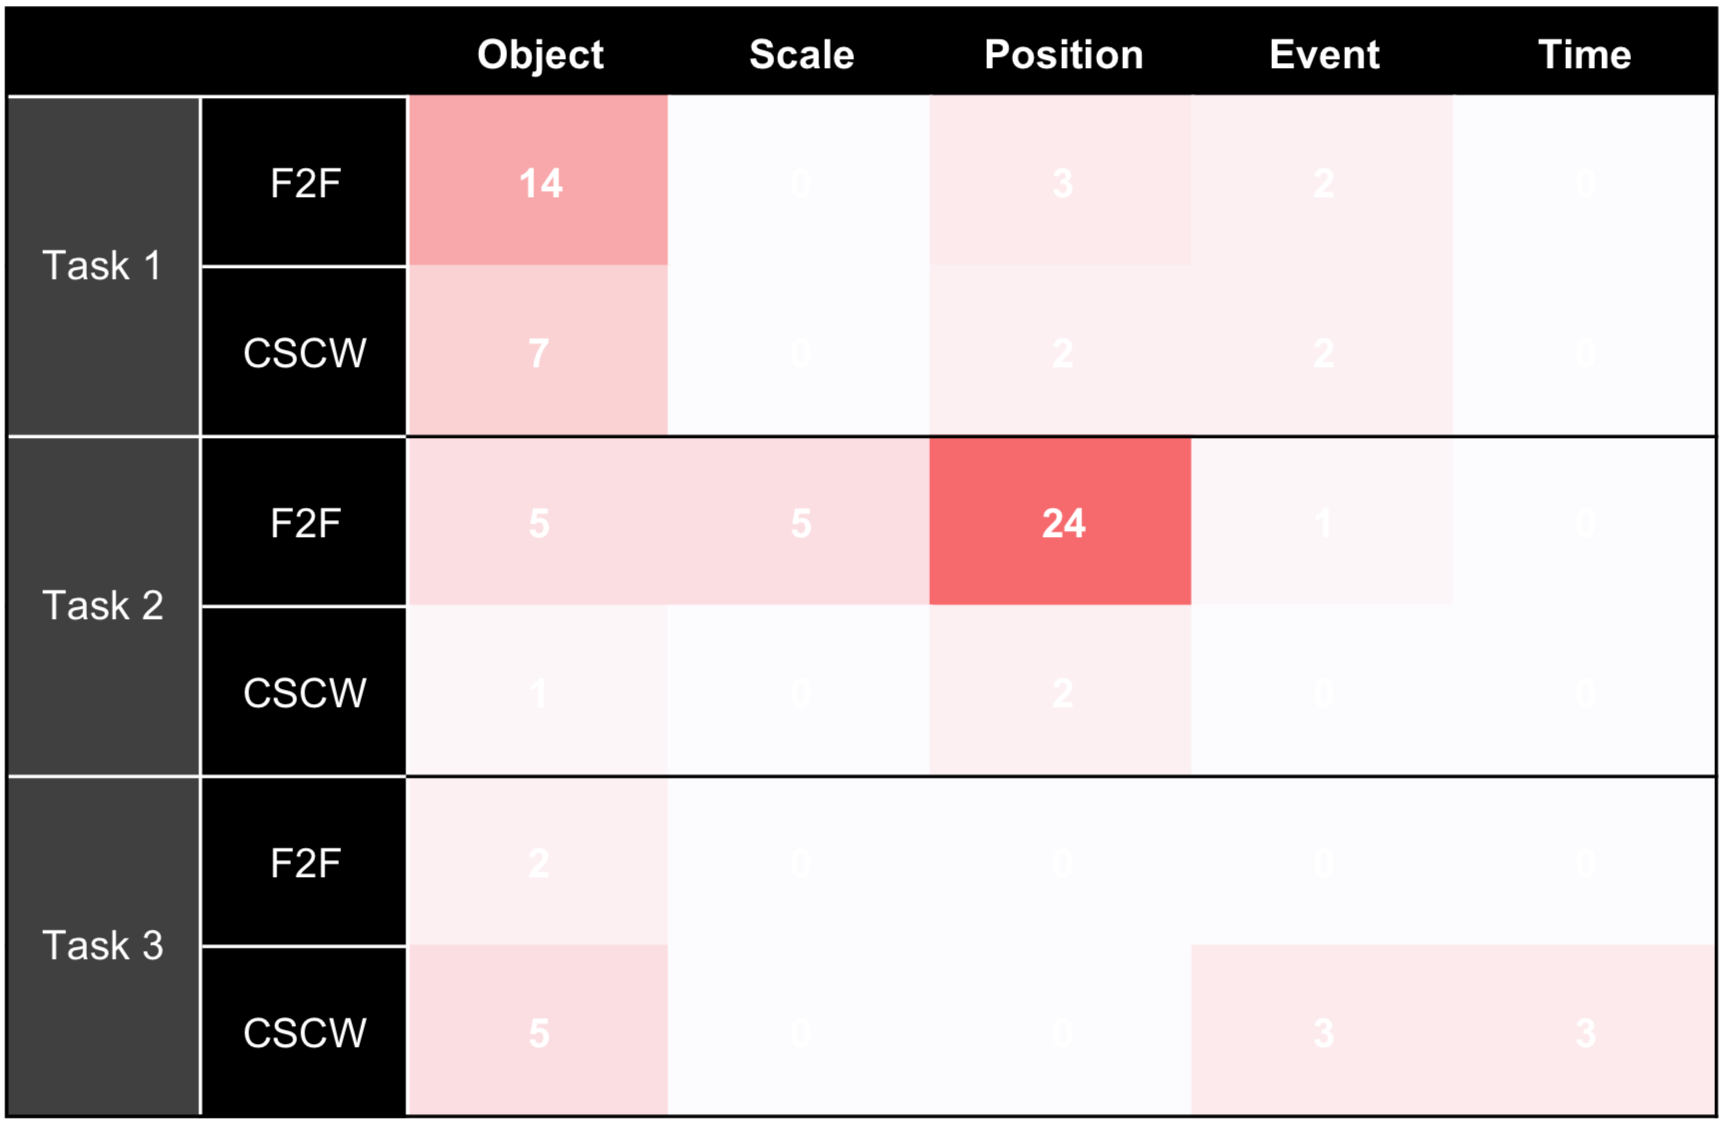
\includegraphics[width = 0.51\textwidth]{deixis_reference_a.png}
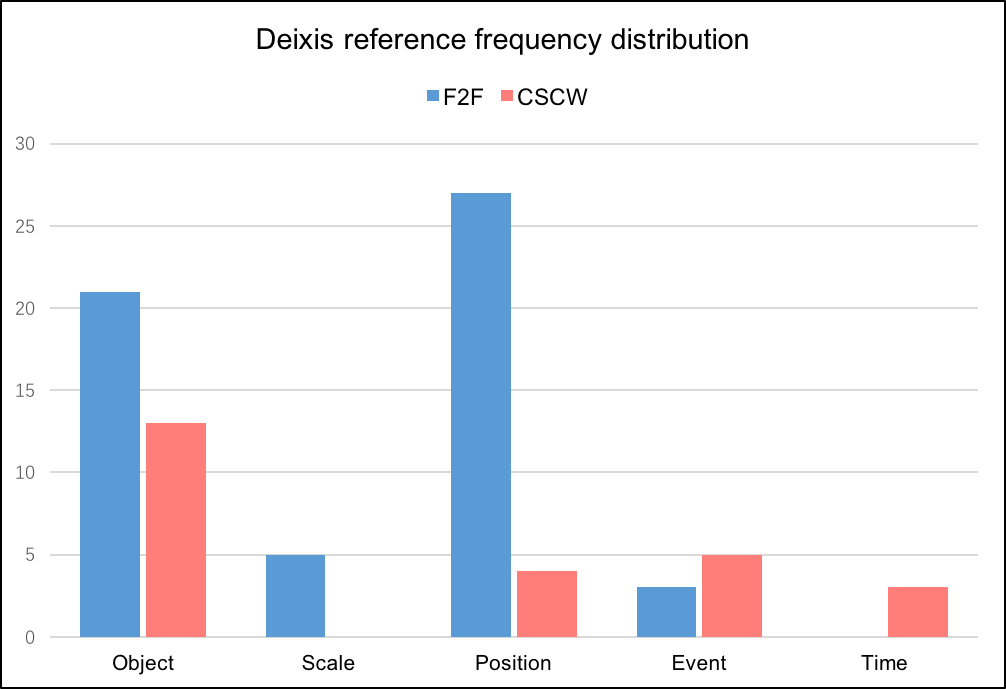
\includegraphics[width = 0.476\textwidth]{deixis_reference_b.png}
\caption{Deixis reference frequency distribution}
\label{Deixis_reference}
\end{figure}

As shown in figure \ref{Deixis_reference}, people use deixis referring to event, time in CSCW is more than in face-to-face. For example, in CSCW collaboration, a person says “I have done my part” to demonstrates his progress. “My part” refers to a event. The most significant thing we can see in figure x is the frequency of position reference. People use deixis to present position is extraordinarily frequent in face-to-face collaboration, especially in task 2, but it is seldom used in CSCW scenario. We observe a episode occurs frequently in face-to-face collaboration: one says “Could we put the window here?” and then point a place on the paper. His collaborator understand what he means and then give a positive confirmation. The figure also shows the most deixis reference used in CSCW is object, and it occurs in task 1 more frequently. Similarly, object as deixis reference also happens many times in face-to-face collaboration. 

\begin{figure}
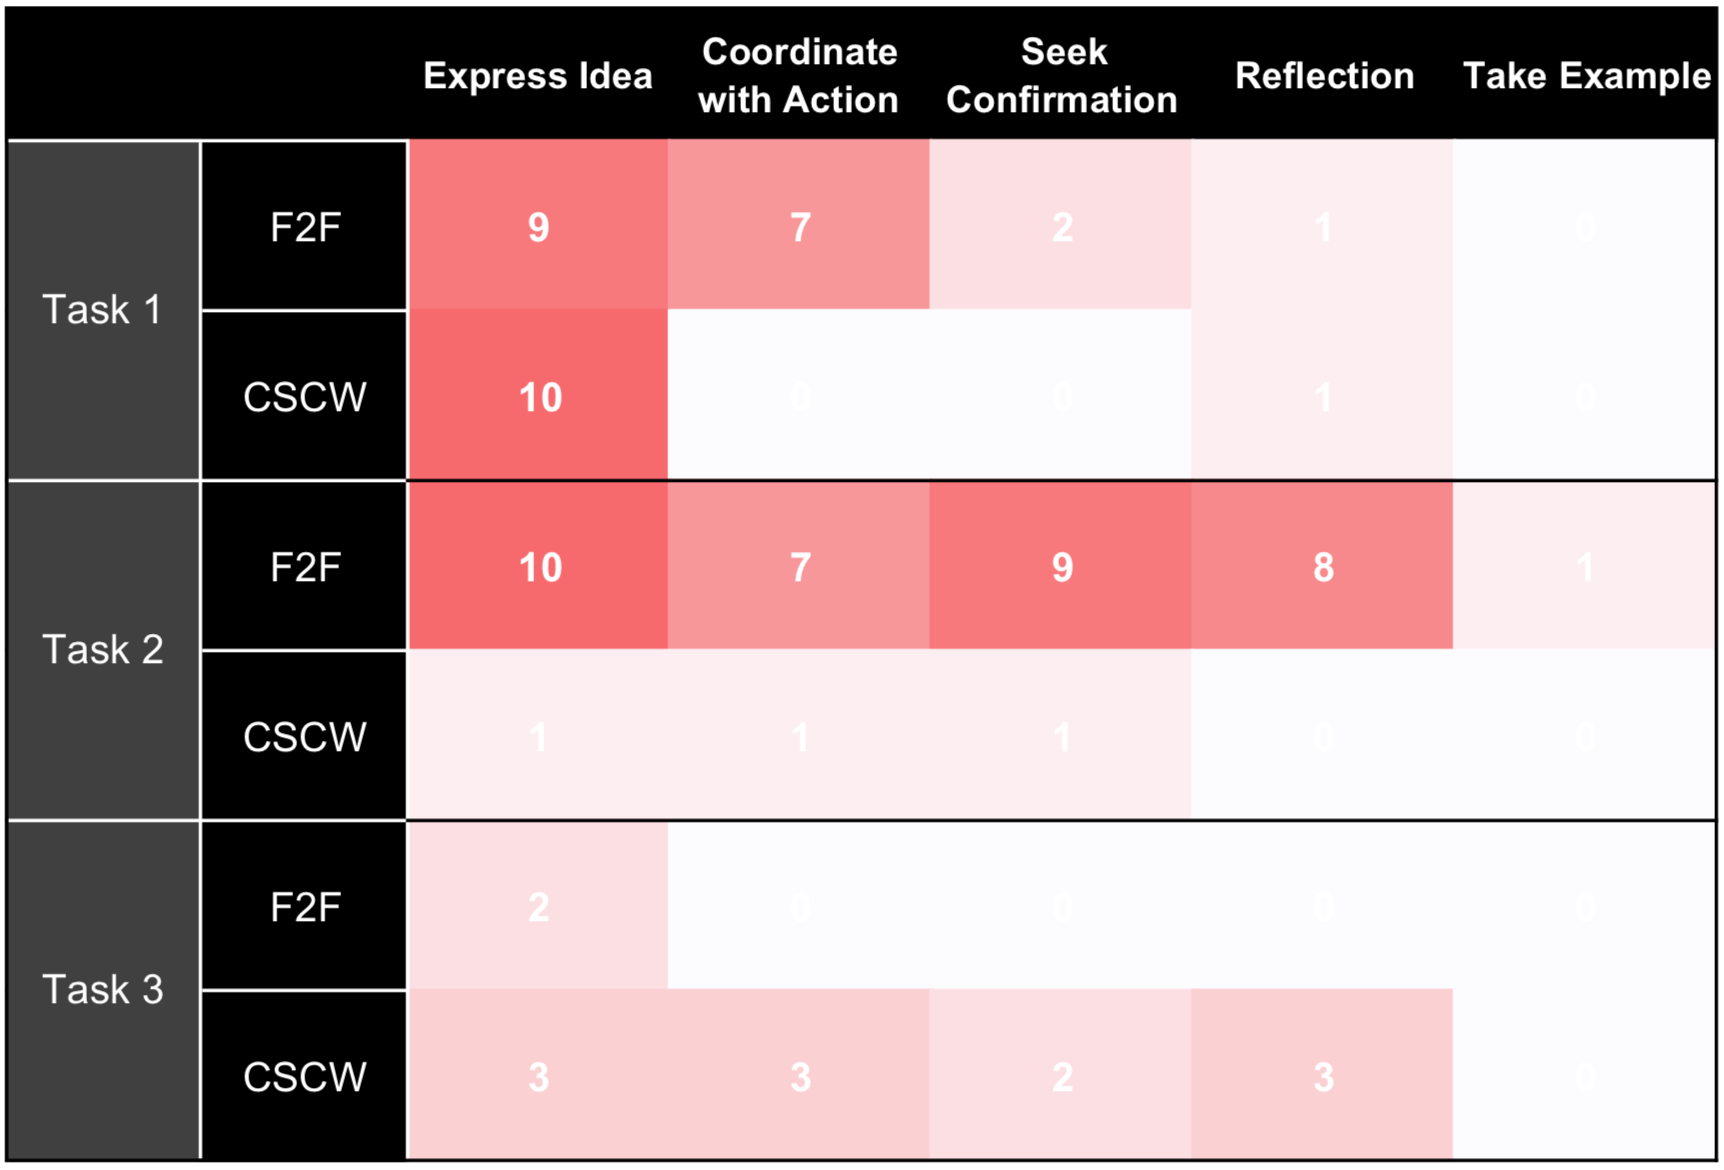
\includegraphics[width = 0.50\textwidth]{deixis_role_a.png}
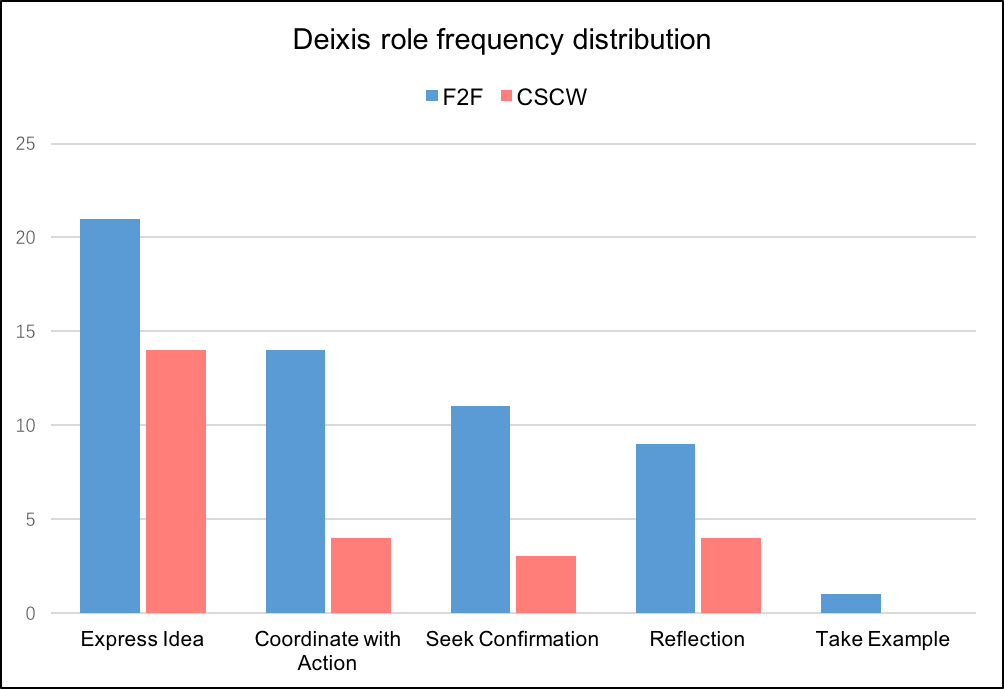
\includegraphics[width = 0.486\textwidth]{deixis_role_b.png}
\caption{Deixis reference frequency distribution}
\label{Deixis_role}
\end{figure}

Figure \ref{Deixis_role} shows the deixis role frequency distribution. In task 2 and task 3, frequency distribution among different roles is relatively average, while in task 1, collaborators tend to express idea and do coordination with deixis. In this figure, we can see that expressing idea is the most important role when using deixis, and in observation we find that such utterance like “The door should be here” to express one’s idea is natural and effective in communication. In addition, people use deixis to coordinate with their action is common as well. For example, when someone are drawing a door on the paper, he will say “The door… should be like that” in the meantime. They use deixis to describe what they are doing. 

\subsection{Prototype}
xxxxxx,xxxxxxx
xxxxx

\section{Discussion}
\label{sec:discussion}
\subsection{User research}
We can see obviously from the results that collaborators are communicating more and using deixis more in the first two tasks, but in task 3, they spends more time in operating and drawing, instead of communication. The reason might be task 3, drawing, is more complicated. It’s require people take time to think how to do composition of a picture, how to use different tools to depict elements, and how to make each element sense, and drawing behaviour is far more complex than move, arrange and sketch. To complete this task, collaborators tend to divide the work at first. After that, they would like to spend more time thinking their own part rather than communicating. We find in the task 3 face-to-face collaboration, people will scan their collaborators, to check the others work and adjust their own progress. However, in CSCW scenario, they are not able to scan other, so they use oral communicate to check and coordinate themselves. That is why frequency of deixis usage of task 3 in CSCW higher than in face-to-face.  In addition, we find that deixis they used in task 3 almost refer to event and time, which are all general reference, rather than specific reference such as object, position. These general reference means people use deixis to coordinate. For example, one person ask “I have done these work, how about you?”, the others should be allowed to notice “these work” meaning then do reaction. The first design implication we extract is that collaborative drawing work groupware should allow collaborators to check other people’s work easily, and coordinate their own work smoothly.\\   
Task 2 requires collaborators do plan and layout in shared workspace. We find that pointing by finger, simple draw to illustrate idea, and using gesture to describe are most frequently action with deixis in face-to-face collaboration of task 2. However, when do same task in CSCW groupware, people’s behaviours are dramatically change: they seldom use deixis with those actions. If we consider pointing, drawing, using gesture are natural in face-to-face collaboration, we can conclude that doing task 2 with CSCW is unnatural, a least collaborators can not execute their familiar and natural action. Currently collaborative drawing groupwares not support these interaction is the reason. The second design implication is from this reason: collaborative drawing work groupware should  support pointing and other hand gesture to enhance communication effectiveness when people use deixis in speaking.\\
Position and object are most frequent deixis reference we find in the user research. The behaviour is quite natural: One say “Put sofa here”, with finger point a position to let his collaborators know where is “here”. But unfortunately, according in our research, position reference has the largest gap between face-to-face and CSCW, which means, the most familiar and natural behaviour used in face-to-face collaboration receives the least support by CSCW groupware. In other word, people intend to use the simplest utterance to express their thoughts. To make communication more efficient, they would use simple hand gesture to assist expression as well. However, this action pattern doesn’t make sense in CSCW scenario, because they will find collaborators can not recognise what they point. This inconsistent between intention and result leads to the next design implication: collaborative drawing work groupware should support to express position, objects, scale and other spatial information when remote collaborators use deixis.\\
In face-to-face collaboration, we find people’s action plays a significant role of orienting collaborators attention. These actions not only assist utterance expression, but also make other people’s focus on current context, meanwhile, offer sufficient contextual information. In CSCW, collaborators can not see other people’s behaviours and reaction simultaneously, thus they lose plenty of contextual information, which is fundamental of using deixis naturally. The direct way to make up missing contextual information in remote collaboration is help collaborators recognise any behaviour respectively. So we conclude the new design implication: collaborative drawing work groupware should allow users notice other collaborators action, gesture, operation result, even facial and expression. 

\subsection{Design implication}
xxxx,xxxxx


\bibliography{II2202-report}
%%\bibliographystyle{IEEEtran}
\bibliographystyle{myIEEEtran}
\appendix
\section{User Tasks in Field Experiment}
\label{appdx:user tasks}

(placeholder: user tasks here)


\end{document}
